\problemname{The Dark Chambers of Chalmers}
You are on your way to the final competition of the Swedish programming olympiad, which is hosted at Chalmers Technical University.
However, you have gotten lost in the university basement.
Your sense of direction is not great, and what makes matters even worse is the very strange design of the basement.

The basement consists of $2 \leq N \leq 1000$ floors.
At the ground level, there is just one large room.
When you go down one floor, the rooms are half as big.
Beneath every room $i$, there are up to two rooms $l_i$ and $r_i$, each exactly half as big as room $i$.
It is possible that only one of $l_i$ and $r_i$ exists, or that both or neither of them exist.
You can move between two rooms through a door if they are directly next to each other,
or through a staircase if one room is directly above the other.


You are currently in some room in the basement, 
and you know that the final competition is hosted in some other room in the basement.
You now want to get to the competition.
Luckily, you have downloaded the app "Campus Maps".
Campus Maps is programmed to find the length of the shortest path to your destination,
where the number of staircases you need to traverse is minimized.
At any point, you can look at the app, and it will tell you this length.

Formally, a path $v$ is some sequence of moves to adjacent rooms.
For any path $v$ from the room that you are currently in to the room where the final is held,
let $A_v$ be the number of times you go through a door, 
and $B_v$ the number of times you go up or down a staircase.
The length of the path is $L_v = A_v + B_v$.
For all possible paths to the final, the app will find those that minimize the value of $B_v$.
Out of these paths, it will choose the one that minimizes the value of $L_v$.
It will then tell you the value of $L_v$.

Since the app is quite slow, you only have time to check it at most $K = 500$.
You also do not have time to pass more than $R = 5000$ rooms.

\begin{centering}
  \begin{figure}[h]
      \centering
      \begin{subfigure}
        \centering
        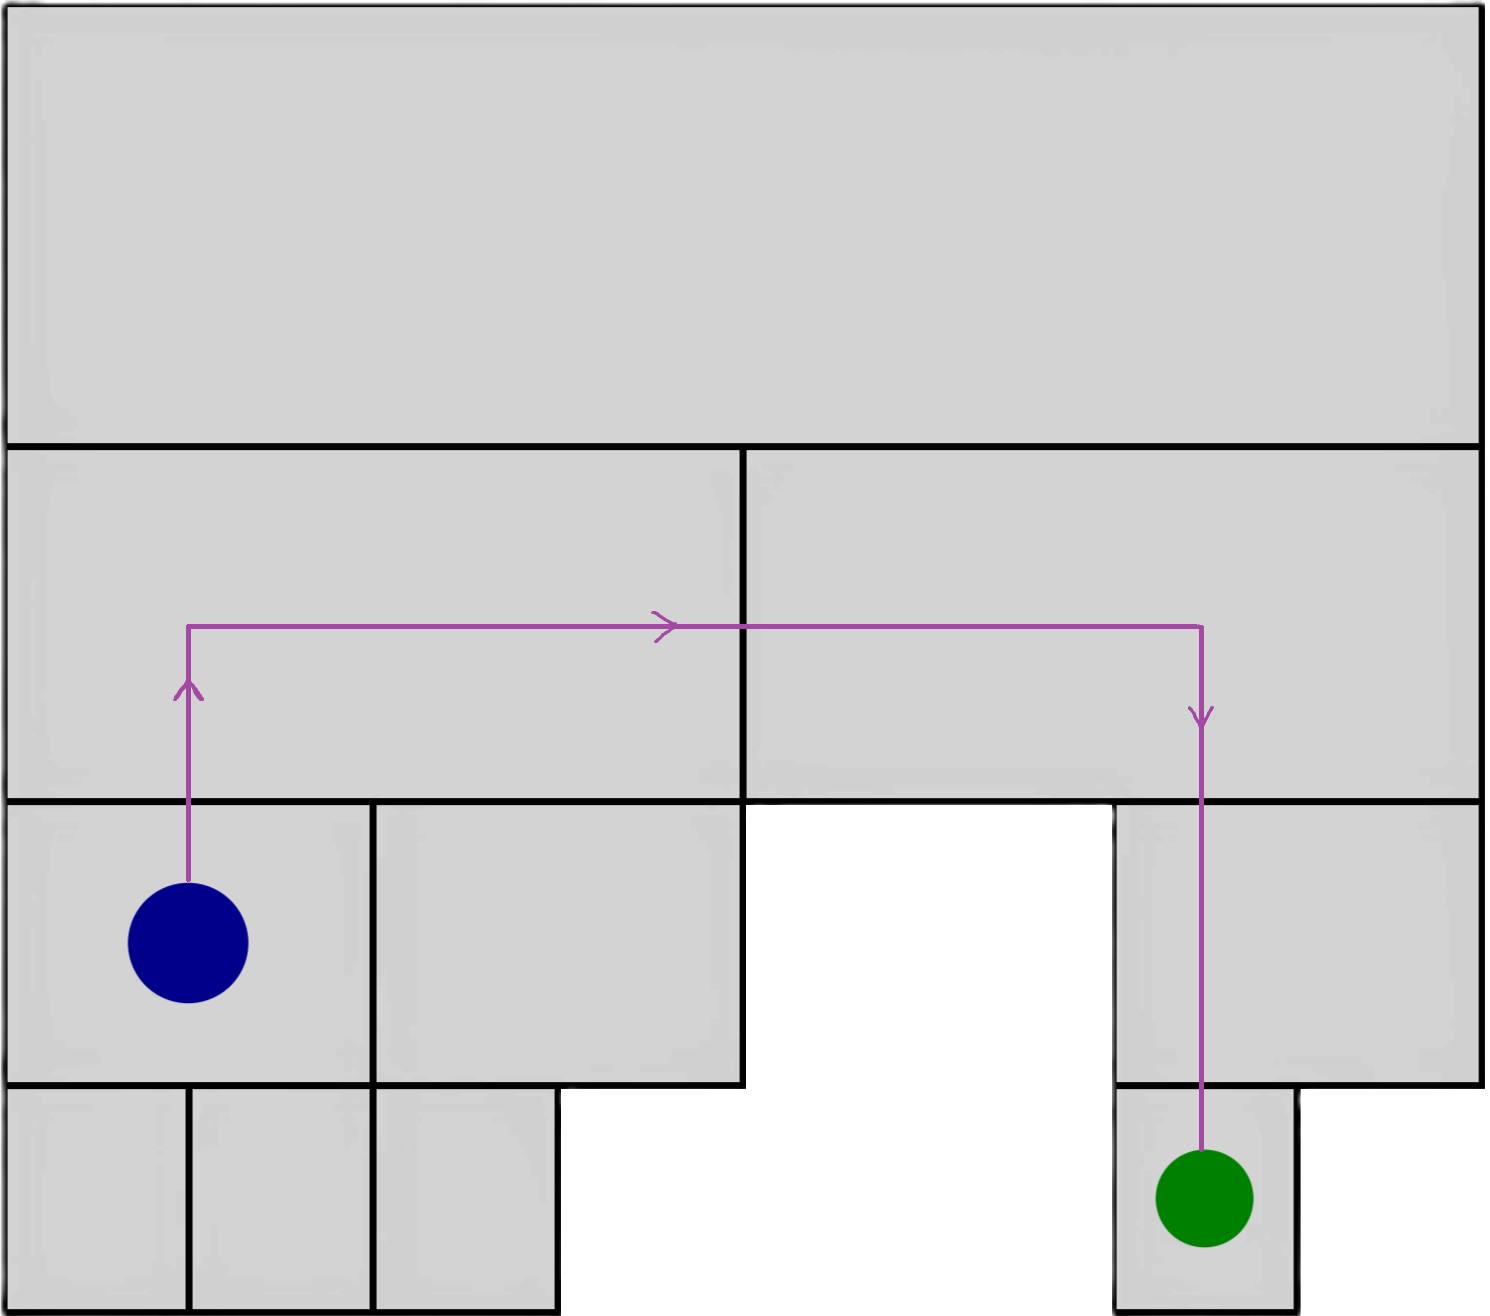
\includegraphics[scale=0.8]{sample1.png}
      \end{subfigure}
      \begin{subfigure}
        \centering
        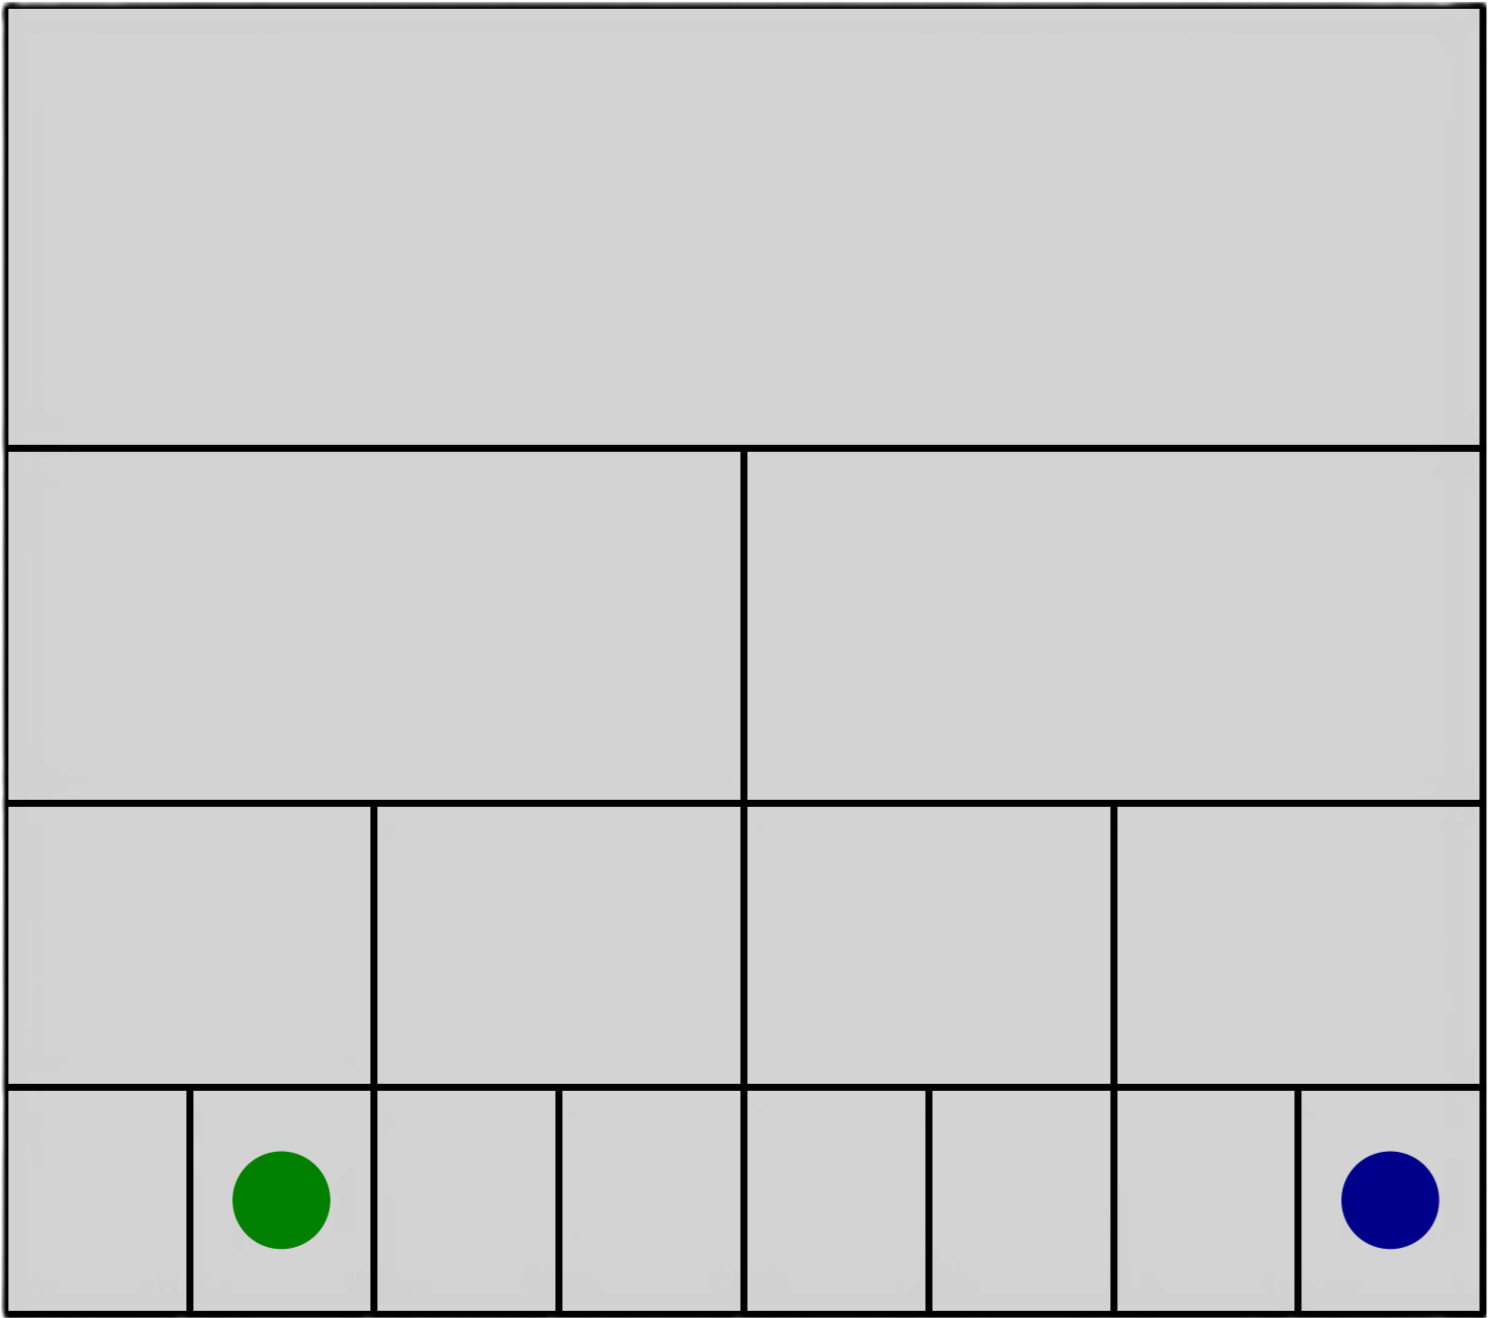
\includegraphics[scale=0.8]{sample2.png}
      \end{subfigure}
      \centering
      \caption{The basement in sample cases 1 and 2. The blue circle is your starting position, and the green circle is the room where the final competition is held.}
      \label{fig:samples}
  \end{figure}
\end{centering}

\section*{Interaction}
First, you get information about the room you are currently in. 
This will be given as a binary string of length five, where every character is '1' if you can go in a certain direction, and '0' otherwise.
In order, the characters tell you if you can go up, right, down to the right, down to the left, and left.
So the string 01001 means that you can go to the right and to the left, but in no other directions.

Then, you choose either to go to an adjacent room, or to use Campus Maps.
To go to an adjacent room you write any of the strings "up", "right", "downright", "downleft", or "left".
Then you get information about the new room you are in, according to the same format as above.

To use the app you write "app".
The app will then calculate the length of the shortest path from where you are to the goal that uses as few staircases as possible.
Since the app is very sensitive to Integer Overflows, it will crash if this length exceeds $10^9$.
In that case, the app will write $-1$.
Otherwise, the length of the path to the goal is written.

When you reach your destination, you should print out "here", and your program should be terminated.


\textbf{Make sure to flush the output after each query}, otherwise you can get \textit{Time Limit Exceeded}.
In C++ this can be done using \texttt{cout << flush}
or \texttt{fflush(stdout)};
in Python with \texttt{stdout.flush()};
and in Java with \texttt{System.out.flush()}.

\section*{Scoring}
Your solution will be tested on a number of sample groups.
To get points in a group your solution must pass all test cases in that group.


\noindent
\begin{tabular}{| l | l | l |}
  \hline
  Group & Point value & Constraints \\ \hline \hline
  $1$   & $10$        & $N = 2$ \\ \hline
  $2$   & $10$        & $N \leq 10$ \\ \hline
  $3$   & $10$        & $N \leq 250$ \\ \hline
  $4$   & $20$        & $N \leq 500$ \\ \hline
  $5$   & $25$        & $N \leq 950$ \\ \hline
  $6$   & $25$        & $N \leq 1000$ \\ \hline
\end{tabular}
